\documentclass[10pt,conference]{IEEEtran}
% \IEEEoverridecommandlockouts
% The preceding line is only needed to identify funding in the first footnote. If that is unneeded, please comment it out.
\usepackage{cite}
\usepackage{amsmath,amssymb,amsfonts}
\usepackage{algorithmic}
\usepackage{graphicx}
\usepackage{textcomp}
\usepackage{xcolor}

\usepackage{listings}
\usepackage{xcolor}



\newcommand\question[1]{{\color{violet}#1}}
\newcommand\todo[1]{{\color{red}#1}}


\definecolor{codegreen}{rgb}{0,0.6,0}
\definecolor{codegray}{rgb}{0.5,0.5,0.5}
\definecolor{codepurple}{rgb}{0.58,0,0.82}
\definecolor{backcolour}{rgb}{0.97,0.97,0.97}

\lstdefinestyle{mystyle}{
    backgroundcolor=\color{backcolour},
    commentstyle=\color{codegreen},
    keywordstyle=\color{magenta},
    numberstyle=\tiny\color{codegray},
    stringstyle=\color{codepurple},
    basicstyle=\ttfamily\footnotesize,
    breakatwhitespace=false,
    breaklines=true,
    captionpos=b,
    keepspaces=true,
    numbers=left,
    numbersep=5pt,
    showspaces=false,
    showstringspaces=false,
    showtabs=false,
    tabsize=2
}

\lstset{
%   basicstyle=\ttfamily,
  mathescape
}



\usepackage{minted}
\usepackage{hyperref}


\bibliographystyle{ieeetr}

\def\BibTeX{{\rm B\kern-.05em{\sc i\kern-.025em b}\kern-.08em
    T\kern-.1667em\lower.7ex\hbox{E}\kern-.125emX}}
\begin{document}

\title{Hardware and Software Co-design for Sparse Linear Algebra Operations Acceleration 
}

\author{\IEEEauthorblockN{Aleksey Tyurin}
\IEEEauthorblockA{\textit{Saint Petersburg State University} \\
Saint Petersburg, Russia \\
alekseytyurinspb@gmail.com}
\and
\IEEEauthorblockN{Daniil Berezun}
\IEEEauthorblockA{\textit{Saint Petersburg State University} \\
\textit{JetBrains Research}\\
Saint Petersburg, Russia \\
daniil.berezun@jetbrains.com}
\and
\IEEEauthorblockN{Semyon Grigorev}
\IEEEauthorblockA{\textit{Saint Petersburg State University} \\
\textit{JetBrains Research}\\
Saint Petersburg, Russia \\
s.v.grigoriev@spbu.ru}
}


\maketitle

%% Abstract
%% Note: \begin{abstract}...\end{abstract} environment must come
%% before \maketitle command
\begin{abstract}

In the era of big data, computations are expected to be faster and less power-consuming in order to become more effective and affordable.
% Sparse linear algebra is a great framework for building algorithms in a uniform and optimization-amenable way.
% However, CPUs and GPUs currently running such algorithms are underutilized due to being too general-purposed for problems that include sparsity.
% Thus, an application-specific integrated circuit could speed sparse computations up, following the example of \textit{Google TPU's}.
% It is worth noting that such a circuit needs to be not self-contained to allow some expected optimizations to be made by a compiler or a framework itself.
% Finally, the optimizations should be easily definable in the language and as automated as possible, thus a careful simultaneous design of hardware and software is needed.
% The proposal describes the bottlenecks inherent to present sparse linear algebra framework implementations, summarizes the expected optimizations, and proposes a co-design approach to designing a highly-optimized sparse linear algebra framework.
% \textit{This is a work in progress and not yet present the final result}.

% While GPU utilization allows one to speed up computations to the orders of magnitude, memory management remains the bottleneck making it often a challenge to achieve the desired performance. Hence, different memory optimizations are leveraged to
% reduce the number of memory transactions and 
% make memory being used more effectively.
%Notably, memory optimizations are being the most significant problem: GPUs memory hierarchy implies certain limitations, thus making data memory allocation management nontrivial and memory to be utilized carefully.
%In the paper we propose an approach automating memory management utilizing partial evaluation, a program transformation technique that enables the data accesses to be precomputed, optimized, and embedded into the code, mitigating memory transactions.
% We propose an approach automating memory management utilizing partial evaluation, a program transformation technique that enables data accesses to be pre-computed, optimized, and embedded into the code, saving memory transactions.
%As an empirical evaluation of our approach we applied the technique to a straightforward CUDA C na\"ive string pattern matching algorithm implementation.
%Our experiments show that the transformed program is up to 8 times as efficient as the original one.
% An empirical evaluation of our approach shows that the transformed program could be up to 8 times as efficient as the original one in the case of CUDA C na\"ive string pattern matching algorithm implementation.   
\end{abstract}


\section*{Introduction}
Linear algebra is a great instrument for solving a wide variety of problems utilizing matrices and vectors for data representation and analysis with the help of highly optimized routines.
And whilst the matrices involved in a vast diversity of modern applications, e.g., recommender systems~\cite{gupta2020architectural,amazon} and graph analysis~\cite{graph1,graph2}, consist of a large number of elements, the major part of them are zeros.
Such a high sparsity incurs both computational and storage inefficiencies, requiring an unnecessarily large storage, occupied by zero elements, and a large number of operations on zeroes, where the result is obviously known beforehand.
The traditional approach to address these inefficiencies is to compress the matrix and store only the non-zero elements. 
Thus, the effect of matrices tending to be sparse in many applications makes the techniques of matrix compressed representation and sparse linear algebra to be the effective way of tackling problems in areas including but not limited to graph analysis~\cite{GAILLA}, computational biology~\cite{compBio} and machine learning~\cite{Kepner_2017}.



Sparse linear algebra defines primitives for expressing algorithms for the mentioned areas in a uniform way in terms of sparse matrix and vector operations parameterized by a semiring.
Such uniform representation allows to tune the whole bunch of expressible algorithms through optimizing the primitives solely.
One of the most used primitive is a sparse matrix-sparse matrix multiplication (spMspM) operation. 
It has finely-tuned implementations for both CPU and GPU, which, however, are proven to be underutilized due to the memory-bound nature of sparse computations induced by compressed representation~\cite{Florida,leskovec2016snap,Song_2016,zhang2020sparch}.
Further, the pipeline of spMspM is patchy, which makes some of the computational units to be idle from time to time as it could be seen in figure~\ref{fig:sm_util}, while the peak FLOPS is less than 1\% of maximum available\footnote{\url{https://hanlab.mit.edu/projects/sparch/} (Accessed 09.02.2021)}. 


\begin{figure}[t]
  \centering
  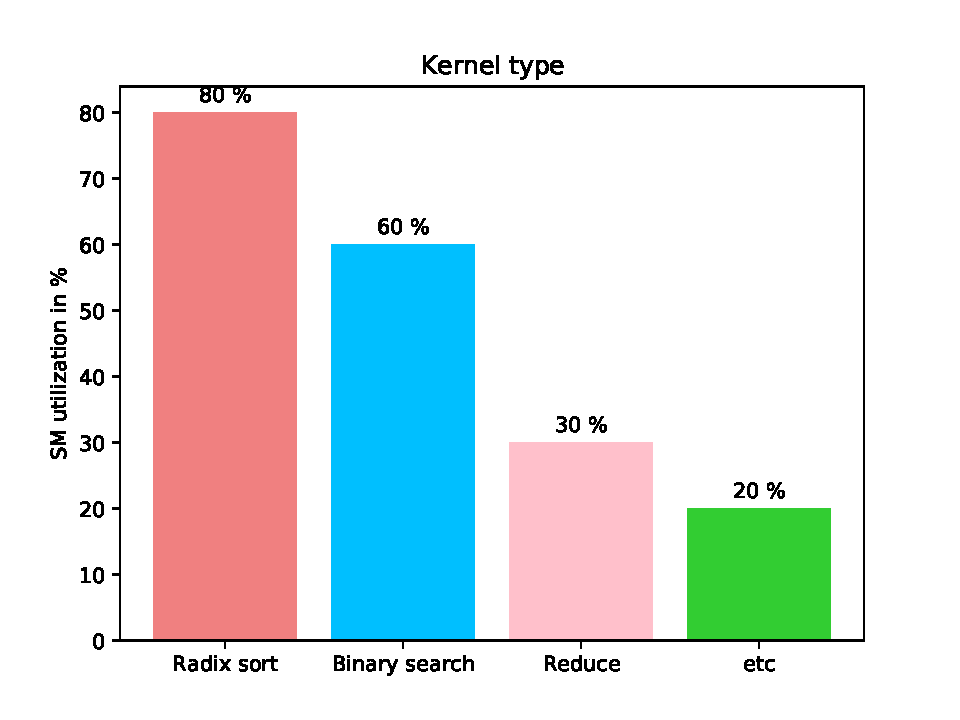
\includegraphics[width=\linewidth]{figs/SM_performance.pdf}
  \caption[Caption for LOF]{GPU's SM utilization for spMspM pipeline from cuSPARSE\footnotemark}
  \label{fig:sm_util}
\end{figure}

\footnotetext{\url{https://developer.nvidia.com/cusparse} (Accessed 09.02.2021)}

\begin{listing}
  \caption{Sequence of sparse operations example}
\label{listing:1}

\begin{minted}[]{haskell}
  -- A,B,C,D are sparse matrices
  -- M is a mask
  D<M> = A eWiseAdd B eWiseMult C
\end{minted}

\end{listing}

This makes the typical CPUs and GPUs not well-suited hardware for sparse computations and gives a rise to specialized hardware accelerators, which are primarily concerned with spMspM.
However, for a sparse framework to be useful, it should incorporate not only spMspM, but also other sparse operations like in listing~\ref{listing:1}, where masking, which filters the matrix elements, and element-wise operations (possibly parameterized by a semiring) needed for, e.g., PageRank and bread-first search (BFS) algorithms~\cite{yang2020graphblast} are presented.
And when such operations are chained explicitly or implicitly, via a loop body, certain optimizations could be applied, like the one that eliminates intermediate matrices in sequence from listting~\ref{listing:1}.
Unfortunately, some of such optimizations (e.g., the one mentioned) are only expressible at software level, i.e., in programming language, hence modern spMspM accelerators could be impractical for accelerating the whole program representing a linear algebra based algorithm like PageRank or BFS, due to the lack of a software part and to a too narrow hardware specialization.
Thus a co-design of dedicated hardware and software components, i.e., domain-specific processor (DSP) and a corresponding domain-specific language (DSL), could provide a system which is not more effecient for spMspM than present hardware accelerators, but appear to be more effective in terms of speed and power consumption for holistic pieces of program, i.e., for chained operations, than current CPUs and GPUs implementations.
The ongoing work is devoted to the design of respective DSL, DSP, and an optimizing compiler, and this work in particular gives a brief overview of the filed, discusses the ideas and challenges behind the design. 



% \emph{Direction-based} optimization is in charge of either deciding to use sparse-vector or dense-vector operations for  matrix-vector multiplication. The current frontier during a graph traversal could grow while the mask of yet not-visited vertices becomes small, so it becomes more profitable to utilize masked dense operations instead of sparse-matrix sparse-vector operations.

% \emph{Load-balancing} optimization chooses the most suitable distribution among the workers (e.g. threads) depending on the sparsity of the operands. Or schedules the operands in a way to save computations, e.g. first merge two small arrays instead of a small and a large array in order to not extend a large array overhead throughout all the computation.

% \emph{Mask fusion}. Ahead-of-time masking could reduce the number of memory accesses in case of matrix-vector multiplication and prevent memory blow-up in case of matrix-matrix multiplication: the multiplication of two sparse matrices could produce an order of magnitude
% more nonzeroes in the output matrix compared with the two input matrices, hence the mask could limit the output number of nonzeroes, thus preventing out-of-memory errors. In order to achieve such a behavior, a mask should be fused (i.e. transformed in a single operation) with the corresponding operation for the operation to perform computations only for the elements in the mask.  

% \emph{Kernel fusion}. Mask fusion is a special case of kernel fusion. Kernel fusion is responsible for fusing arbitrary operations. In the case of functional programming fusion~\cite{fusion} could be thought of as eliminating allocation of intermediate values of function composition, most notably for lists, since they are the primary data structure of functional programming. In the listing~\ref{listing:3} append function \texttt{app} joins three lists, and fusion generates such code for function \texttt{f} that traverses each list only once. A simple motivating example for kernel fusion could be seen in listing~\ref{listing:2}. Masking, addition, and subtraction could be fused in one kernel code to prevent intermediate results allocation and redundant memory accesses for traversal for each or element-wise operation. The graph representation of operations could exploit operation properties, e.g., associative property, to perform the fusion. Further, the fusion for operations that could be represented as a composition of \texttt{map/reduce} operations are well-studied and could be effectively fused~\cite{KernelFusion,Futhark}.
% \begin{listing}
% \centering
% \caption{Fusion of function composition}
% \label{listing:3}
% \begin{minted}{haskell}
% app [] ls = []
% app (x:xs) ls = x : app xs ls

% -- call for this function

% app xs (app zs ys)

% -- is fused to the following function definition
% -- that is specialized for three lists

% f [] xs ys = g xs ys
% f (x:xs) ys zs = x : f xs ys zs

% g [] xs = xs
% g x:xs ys = x : g xs ys

% -- and a call
% f xs zs ys

% \end{minted}

% \end{listing}
% % \begin{minted}[escapeinside=||]{haskell}
% % map f (map g list) |$\equiv$| map (f |$\circ$| g) list 
% % \end{minted}


% \begin{listing}
% \centering
% \caption{Kernel fusion example}
% \label{listing:2}
% \begin{minted}{python}
% #Fusing together '+', '-', and masking
% #prevents two intermediate matrices allocation

% C<mask> = A + C - B
% \end{minted}
% \end{listing}

% \emph{Specialization}. Generally, it is a program transformation optimization~\cite{jones} that exploits the knowledge of some of the operation parameters, hence it could optimize those parts of the operation that depend on the known pieces of information. In the case of \emph{NVIDIA CUDA} specialization assigns a specialized computation per a warp, since warps could be executed independently. This technique is well-described, e.g.,  in~\cite{CUDADMA}. An example of such optimization could be a matrix-vector multiplication in some cycle where the vector remains unchanged. Hence, the vector could be embedded in the operation itself avoiding vector-specific overheads, e.g, allocation or data transfer back-and-forth from host to device. Matrix-vector multiplication is essentially a linear combination of columns where each column has a corresponding coefficient from the vector. Thus, each warp could multiply it's assigned column by the \texttt{warp\_id's} element of the vector, which could be embedded in the code of the warp itself. Such embedding is generally a huge \texttt{warp\_id} \texttt{switch} statement, which incurs almost no overhead in the case of CUDA.

% However, there are inevitable challenges both for the hardware running sparse algorithms and for the software, performing optimizations. 

% For the former, both CPUs and GPUs remain underutilized when executing sparse operations due to high cache-miss rates, limited communication between processors~\cite{Song_2016}. Sparse algorithms are inherently memory-bound and thus results in poor GFLOPs number compared to peak GFLOPs theoretically available on modern devices, namely less than $0.2\%$ of theoretical performance is achieved as reported in~\cite{leskovec2016snap, Florida}.

% For the latter, optimizations are hard to automate and perform in general. The runtime of graph kernels is dependent on the input data, so in a multiple iteration algorithm, it might be profitable to fuse two kernels in one iteration and two different kernels in a different iteration. Further, kernels are compelled to satisfy certain restriction to be fuseable: the absence of intermediate synchronization, same data access pattern, enough resources on the device to execute fused kernel. Once again, \texttt{map/reduce} kernels could be successfully fused, but it is unclear whether GraphBlas standard could be solely implemented in \texttt{map/reduce} terms. For specialization, it is better for the underlying hardware to be \emph{MIMD} for the workers to be completely independent, however GPU's architecture is \emph{SIMT} (or \emph{SPMT}), which prevents successful specialization in many cases.

% Eventually, some application-specific integrated circuits have been designed to address the issues mentioned above, that basically provide hardware units for sparse matrix-matrix or matrix-vector multiplication~\cite{zhang2020sparch, Song_2016, Systolic,CPU-FPGA}. A brief overview could be found in~\cite{zhang2020sparch}. The implementation from~\cite{zhang2020sparch} greatly outperforms CPUs (Intel MKL\footnote{\url{https://software.intel.com/content/www/us/en/develop/tools/oneapi/components/onemkl.html}}) and GPUs (cuSPARSE\footnote{\url{https://developer.nvidia.com/cusparse}}) solutions in terms of speed and power consumption. Despite high performance, such solutions do not yet provide a complete implementation of GraphBlas (or even a subset required for a concise BFS from the example) and seem to be too self-contained to split the operation into phases that could be optimized in the discussed sense. 

% Thus, a solution that combines the hardware and software in co-design fashion considering both hardware and software bottlenecks could be proposed. 
% The hardware should be general enough to allow software optimizations and the optimizations should be easily definable in the co-designed language. 
% A possible approach to tackle the design problem is to use a co-design framework~\footnote{\url{http://openasip.org/}} and TTA processor architecture, which is highly parallel and customizable (allowing, e.g., MIMD computations). 

% Currently, sparse algebra frameworks speed up graph data\-bases, e.g., RedisGraph~\footnote{https://oss.redislabs.com/redisgraph/}, computational biology and machine learning, and equipping cloud solutions that provide such services with the dedicated sparse hardware could both increase the performance of the queries and make the services more affordable by reducing power consumption following Google's TPUs~\footnote{\url{https://cloud.google.com/tpu}} example.   

\section{Problem statement}
Since sparse linear algebra applications are mostly concerned with graph problems, some of the optimizations are graph-specific~\cite{yang2020graphblast,graphIt}, e.g., direction optimization.
However, in memory-bound applications optimizations that minimize data transfer are essential. 
For example, \emph{kernel fusion} is a wide addressed optimization that fuses multiple operations into one, avoiding intermediate memory accesses, utilizing, e.g., registers to pass the data between the operations.
In the case of sparse linear algebra frameworks kernel fusion is not yet widely implemented, but most often related to fusing chained operations like
% \begin{minted}[escapeinside=//]{haskell}
%   D<M> = A eWiseAdd B eWiseMult C
% \end{minted}
from listing~\ref{listing:1} to avoid intermediate matrices construction and reduce memory accesses with masking~\cite{yang2020graphblast}.

The problem of intermediate data structures is common for functional programming
and there have been developed a number of 
optimization techniques that try to reduce intermediate 
data structures or computations, namely partial evaluation~\cite{jones}, deforestation~\cite{WADLER1990231}, supercompilation~\cite{supercompilation}, and distillation~\cite{distillation}.

These fusion family optimizations are implementation-dependent, meaning that the optimizer should have an access to the source code, which is impossible when the function is implemented solely in hardware, hence a software part is inevitable in the design of a systems that tries to put together fusion and hardware.
Thus, present hardware accelerators are not general enough to implement and accelerate a whole sparse linear algebra-based program, e.g., do not provide arbitrary semiring support, and lack a software part hence leaving out essential optimizations.
General purpose devices such as GPUs are hard to perform some optimizations, e.g., fusion requires two GPU kernels to have the same memory access pattern and partial evaluation could induce some thread divergence due to SIMD nature of a GPU. 
Further, present systems that support fusion are domain-specific\footnote{\url{https://www.tensorflow.org/xla} (Accessed 09.02.2021)}, or perform the optimization on top of data structures that may not be suitable for sparse operations (mainly for effective compressed representation), e.g., streams and lists~\cite{StreamFusion,StreamFusion2}, while array-based fusion systems does not perform fusion with index arithmetic~\cite{Futhark}.
Finally, some data needed for optimizations~\cite{jones} is only available in runtime, thus there should be support for JIT optimizations.
The design of the proposed hardware-software system should take these challenges into consideration. 
Next, we discuss hardware accelerators from adjacent areas and elaborate about the software optimization we want to exploit.
% \question{
% We propose the co-design of \todo{???} to address the problems of optimizeability and expressibility.
% We believe that a functional DSL, where an arbitrary semiring could be concisely and conveniently expressed, powered by a set of optimizers and compilable to some DSP with enough parallelism could be a good starting point in acceleration of sparse linear algebra based programs.
% Next we discuss some possible hardware architectures and incurred challenges as well as high-level architecture of the proposed solution.
% }

% LA but whole program optimization.
% Fusion and so on.

% \todo{Static vs dynamic data.}
% \todo{Specialization requires MIMD.}

% \todo{Representation for data (formats)}

% \todo{AOT vs JIT optimizations.} 
% \todo{Some data become static in running time.} 


% \section{Sparse LA arch}

\section{Graph processors}
Sparse linear algebra is often concerned with graph problems, and since
graph processing is mature enough to be considered as a distinct computation paradigm, there have been emerged a number of graph processors~\cite{GraphProcessors} to mitigate the issues of graph processing on general-purpose processors.
However, many proposed accelerator models are not generic, in the sense they are optimized for specific
classes of graph algorithms and lack scalability. Further, sparse linear algebra makes graph computations more amenable to effective parallelization, ease scalability and even spreads beyond graph computations~\cite{compBio}. 
Presently, there is no sparse linear algebra-based instruction set processor~\cite{Song_2016},
while other sparse linear algebra accelerators~\cite{CPU-FPGA,OuterSpace,zhang2020sparch} are applicable only to certain operations like spMspM.
Notably, in~\cite{smash} the way of compressed representation of a sparse matrix is identified as the main bottleneck and an approach for hardware acceleration for compressed representation indexing is proposed, which is able to employ existing optimizations and could be integrated into existing software frameworks.
Hence, the underlying hardware is better to support the indexing needed by a compressed representation of choice to be effective.
However, we believe that to fully leverage fusion the indexing should be transparent, i.e., constructive, in the software, which is not the case in~\cite{smash}.

\section{Partial evaluation and supercompilation}
Since intermediate data structures are incurred by the concept of functional programming, a lot of techniques have been developed to reduce the number of such structures and the number of computations in general.
Supercompilation~\cite{supercompilation} could be thought as a combination of many such optimizations~\cite{distillation,WADLER1990231,jones}.
In particular, partial evaluation~\cite{jones} stands for precomputing the parts of a program that depend on statically known data. interestingly, some data may become static in runtime, e.g., it could remain fixed between different iterations of a loop, thus it may be profitable to perform such optimization even in runtime.
Despite such optimizations are common in the world of functional programming, they are hard to perform in case of imperative languages widely used in high performance computing.
However, a fully working supercompiler at the moment is developed only for a small functional language, since being too hard to implement for a rich language like Haksell. But we believe that such a small language is enough to provide a DSL for sparse linear algebra.
Also, such optimization may produce a burden of \texttt{case} statements, which slow down the hardware that exploits SIMD model, hence they could not be executed in parallel.
Finally, fusion performed, e.g., by a supercompiler heavily depends on the compressed representation, i.e. presently quad tree representation seems to fit more for fusion than, e.g., coordinate format. 
Some operations could not be fused in principle, e.g. sorting, but the need for some of such operation could be induced by the compressed representation once again, e.g., quad tree representation does not require sorting, so it is reasonable to implement non-fusable operations in hardware.

% Partial cases for different models (array programming, stream fusion, kernels fusion)

 
% We can use small language to design LA library.

\section{Functional language processors}
The functional DSL is not of much use until effectively compiled for DSP.  
There are a number of works that aim to add a hardware support for functional programming~\cite{ACqua,Reduceron,PILGRIM}. Where \cite{ACqua} leverages the parallelization of independent function calls, which do not appear much after supercompilation~\todo{True or not? More likely False}, and also
provides an optimized support for lists and \texttt{map} operation specifically, which may not be the desired property due to the compressed representation of choice. Further, the general-purpose nature of such processors could hurt sparse operations performance due to non-specialized cache.
They also focus on hardware support for graph reduction via parallelization, specialized memory, and pipelining, thus even more parallelism could be extracted from compressed representation.
However, present functional processors could be too complex to integrate with, e.g., to add hardware support for indexing or another computation that cannot be optimized effectively in software. 
Instead, we plan to leverage the approach of dataflow representation of functional programs with indirect memory accesses~\cite{funcHLS}, which then could be effectively represented in hardware in a highly parallel way. 
The approach currently generates application-specific RTL code, but we hope to adapt it for dataflow processor architecture, e.g., transport-triggered-architecture (TTA), in order to have highly scalable and parallel processor with hardware support for a compressed representation, able to run functional programs and easily extensible with custom operations. 

% Thus, we need to explore the potential of different compressed representations in terms of hardware support and fusion. A prominent candidate is a quad-tree representation, which is more amenable to supercompilation (and hence to fusion), \todo{while a program after supercompilation basically represents a dataflow through pattern matching and semiring operations}.

% An interesting feature of functional languages is that they could be compiled to dataflow representation~\cite{funcHLS}, which could be implemented in hardware with high parallelism and scalability. With this approach a program is compiled to it's specific hardware description, but we hope to put together a highly parallel and scalable dataflow processor architecture, e.g. transport-triggered-architecture, hardware support for the compressed representation, and a functional domain-specific language.
% \section{Dataflow processors}

% \todo{Nothing except TTA :(}
% TTA and other dataflow + MIMD

\section{Research Questions and Roadmap}

As a result, we think that solution should includes simultaneous design the following components.
\begin{itemize}
  \item Functional domain specific language to develop a library of sparse linear algebra operations. 
  Functional programming language is well-suitable for supercompilation and for specialized hardware creation.
  THe language should be minimized to simplify optimizations and comilation, but expressive enough to implement almost all GraphpBLAS specification.
  \item Compiler form the functional DSL to the specialized hardware. 
  \item Supercompiler for the functional DSL. Supercompiler should be designed for multistage processing.
  For example, first stage is a compile-time fusion of functions, and the second stage is a specialization on some data. 
  This allows one to exploit dynamic data as static, and minimize overhead in running time. 
  \item Library of sparse linear algebra operations (GraphBLAS implementation) in the functional DSL.
  We should to choose such representation of vectors and matrices, and such principles of code design, that both, required software optimizations and efficient hardware design should be possible.  
  \item Special hardware which should be general enough to execute all code written in the functional DSL with utilization of the library of linear algebra operation.  
\end{itemize}

Such the multicomponent solution with nontrivial connections between components requires deep analysis in number of areas.
So, at the first stage we plan to focus on the following questions.
\begin{enumerate}
  \item Is supercompilation suitable for required optimizations? For example, can it remove intermediate matrices creation in chained operations, like presented in listing~\ref{listing:1}.
  \item Can we generate program-specific hardware from the linear algebra operation written in functional programming language such that it will be efficient in comparison with current solutions?
  \item Is supercompilation suitable in functional-program-to-hardware workflow? Does supercompiled program compiles to more efficient hardware that original one?
  \item Does staged supercompilation allow to minimize specialization time enough to apply specialization in running time? 
\end{enumerate}

As a first step we plan to write prototype of some operations like multiplication, element-wise addition, Kronecker product, and masking in minimalistic functional programming language (Haskell-core) and try to apply HOSC~\cite{!!!} to it. 
It allows us to estimate supercomilation effect in terms of expected optimizations like fusion, and time required for specialization. 
Also, at his step we should establish principles to design the library to maximize supercompilation effect.

At the same time we plan to evaluate functional language to hardware compiler~\cite{funcHLS} on the developed library to estimate performance of implemented operations and to compare basic and supercompiled versions.

As a result of this step we expect to estimate an applicability of functional programming language and related optimization techniques to crate high-performance linear algebra based solutions. 
As a result we should to provide a solution for program-specific accelerators creation for sparse linear algebra based subprograms. 

As far as the final goal is to create not program-specific hardware accelerator, but a processor unit for high-performance linear algebra based computations, the second stage should be focused on the flowing strongly connected questions. 
\begin{enumerate}  
  \item Can generalize ideas from functional languages to hardware compilation to create a specific processor unit for sparse linear algebra?
  \item Can the designed language be efficiently compiled to the designed processor unit?
\end{enumerate}

As a result of this stage we hope to cerate a specialized processor unit for sparse linear algebra and a compiler from the functional DSL to it.


The final stage is a creation of SDK to integrate the DSL to application. 
The SDK should provide tools for staged optimizations, communication with the special processor unit, interoperability with general-purpose programming languages. 


%% Bibliography
\bibliography{bib}


%% Appendix
% \appendix
% \section{Appendix}

% Text of appendix \ldots


\end{document}